\section{Benchmarks}
We compared the running times of Acme++ and the previous
implementation AcmeML to justify this upgrade. We report the results
in this section.

For the benchmarks we randomly chose automata which produce larger
Markov monoids in order to observe the difference in performance
between the two versions. The point of comparison is the size of the
computed monoid rather than the number of states in the automaton,
since some large automata can indeed produce small monoids, and
vice-versa, some small automata can produce large monoids.

To this extent, for each state $s$ we pick a state $t$ with uniform
probability on the set of states and add a transition between $s$ and
$t$. After this we uniformly pick a number $p\in[0,1]$, and for all
other states $t'$ different from $t$, we decide whether we will add a
transition between $s$ and $t'$ by flipping a $p$-biased coin.

The results have been plotted in Fig. \ref{bench1}. 

If for some sizes of the monoid in the x-axis there is no
corresponding point for the AcmeML implementation, it means that it
either timed out or had a stack overflow.

\begin{figure}[h!]
  \label{bench1}
  \begin{center}
    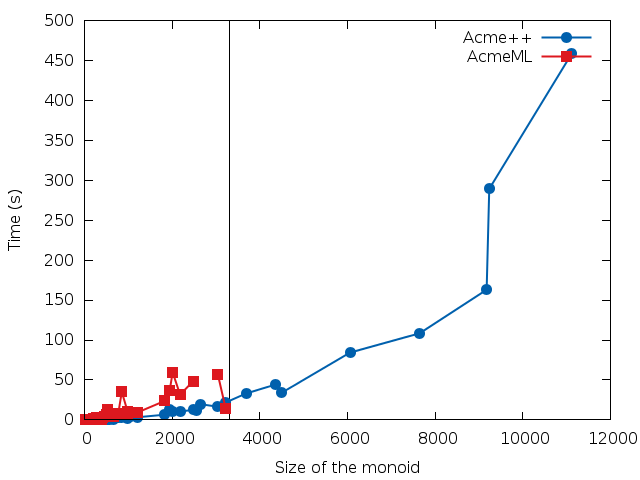
\includegraphics[width=0.8\textwidth]{graph/lines}
    \caption{The time it takes for the two implementations to
      calculate the Markov monoids generated by randomly picked
      automata of size 10}
  \end{center}  
\end{figure}

One can observe that there is a threshold in the size of the Markov
monoid after which AcmeML will not be useful, i.e. it will either take
too much time or have a stack overflow. This threshold is expressed by
the vertical line in the graph above (it hovers around 3500 elements).

Even on smaller examples Acme++ outperforms AcmeML by a considerable
factor as seen in Fig. \ref{bench1zoomed}.

\begin{figure}[h!]
  \label{bench1zoomed}
  \begin{center}
    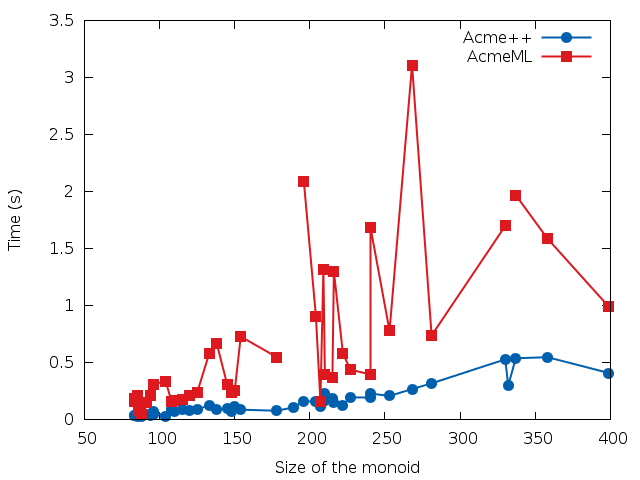
\includegraphics[width=0.8\textwidth]{graph/zoomlines}
    \caption{The same experiment as in Fig.\ref{bench1} on automata
      generating smaller Markov monoids}
  \end{center}  
\end{figure}
